\documentclass{article}

\usepackage{arxiv}
\usepackage[utf8]{inputenc} 
\usepackage[T1]{fontenc}
\usepackage{newunicodechar}
\newunicodechar{́}{\'{}}    
\usepackage{hyperref}       
\usepackage{url}            
\usepackage{booktabs}       
\usepackage{amsfonts}       
\usepackage{nicefrac}
\usepackage{graphicx}
\usepackage{subcaption}
\usepackage{verbatim}
\usepackage{adjustbox}
\usepackage{float}
\usepackage[spanish]{babel}
\usepackage{microtype}      
\usepackage{lipsum}
\usepackage{amsmath}
\graphicspath{ {./images/} }
\renewcommand{\refname}{Referencias}
\usepackage{caption}


\title{TP 2.1 - Generadores Pseudoaleatorios }


\author{
 Aldana Risso Patrón \\
  Universidad Tecnológica Nacional - FRRO \\
  Zeballos 1341, S2000, Argentina \\
  \texttt{rissopatronaldana7@gmail.com} \\
   \And
 Ignacio Fierro \\
  Universidad Tecnológica Nacional - FRRO \\
  Zeballos 1341, S2000, Argentina \\
  \texttt{nachofier@gmail.com} \\
  \And
 Lucía Gelmetti \\
  Universidad Tecnológica Nacional - FRRO \\
  Zeballos 1341, S2000, Argentina \\
  \texttt{luligelmetti@gmail.com} \\
  \And
 Juan Cruz Bonanno \\
  Universidad Tecnológica Nacional - FRRO \\
  Zeballos 1341, S2000, Argentina \\
  \texttt{bonanno2340@gmail.com} \\
  \And
 Franco Reggiardo Chuglar \\
  Universidad Tecnológica Nacional - FRRO\\
  Zeballos 1341, S2000, Argentina \\
  \texttt{francoreggiardo15@gmail.com} \\
  \And
 Marcos Oldani \\
  Universidad Tecnológica Nacional - FRRO \\
  Zeballos 1341, S2000, Argentina \\
  \texttt{marcosoldani1360@gmail.com} \\
}

\begin{document}
\maketitle
\begin{abstract}
El siguiente documento tiene por objetivo detallar el trabajo de clase que debe realizarse para
introducirnos en uno de los elementos fundamentales para gran parte de las simulaciones, esto son
los generadores de números pseudoaleatorios.
\end{abstract}

\keywords{Simulación \and Generadores de numeros \and Análisis Estadístico \and Numeros aleatorios \and Numeros pseudoaleatorios }

\section{Introducción}
La aleatoriedad se entiende como un proceso en el cual el resultado es completamente imprevisible y depende únicamente del azar. Esta característica hace que la generación de números verdaderamente aleatorios sea una tarea compleja, ya que requiere el uso de factores externos incontrolables que aporten esa imprevisibilidad. En contraste, los números pseudoaleatorios son generados mediante algoritmos deterministas que, aunque producen secuencias sin patrones evidentes desde un punto de vista estadístico, no son verdaderamente aleatorios. Bajo las mismas condiciones iniciales, estos algoritmos generan siempre la misma secuencia de números. A pesar de esta limitación, los números pseudoaleatorios resultan extremadamente útiles en diversos campos, especialmente en estos trabajos de estudio de la simulación, donde su comportamiento estadísticamente aleatorio es suficiente para modelar fenómenos complejos.


\section{Generadores de numeros}
\subsection{Generadores de numeros aleatorios reales}

Los números completamente aleatorios (no
determinísticos) son fáciles de imaginar conceptualmente, por ejemplo podemos imaginar
lanzar una moneda, lanzar un dadoo una lotería.
En general los números aleatorios se basan en alguna fuente de aleatoreidad física que
puede ser teóricamente impredecible (cuántica) o prácticamente impredecible (caótica). 
La desventaja de éstos métodos es que son costosos, tardados y no reproducibles.

\subsection{Generadores de números pseudoaleatorios}

Los números pseudoaleatorios se generan de manera
secuencial con un algoritmo determinístico, formalmente se definen por:
Función de inicialización. Recibe un número (la semilla) y pone al generador en su estado inicial.
Función de transición. Transforma el estado del generador.
Función de salidas. Transforma el estado para producir un número fijo de bits (0 ó 1).
Una sucesión de bits pseudoaleatorios se obtiene definiendo la semilla y llamando repetidamente la función de transición y la función de salidas.

Esto implica, entre otras cosas, que una sucesión de números pseudoaletorios esta completamente determinada por la semilla.

\subsubsection{Método de los cuadrados}

En 1946 Jon Von Neuman sugirió usar las operaciones aritméticas de una computadora para
generar secuencias de número pseudoaleatorios.
Sugirió el método de los cuadrados (middle square), para generar secuencias de dígitos pseudoaleatorios de 4
dígitos propuso:

\begin{enumerate}
    \item Se inicia con una semilla de 4 dígitos. 
    \item La semilla se eleva al cuadrado, produciendo un número de 8 dígitos (si el resultado tiene menos de 8 dígitos se añaden ceros al inicio). 
    \item Los 4 números del centro serán el siguiente número en la secuencia, y se devuelven
como resultado.
\end{enumerate}

Este generador cae rápidamente en cilcos cortos, por ejemplo, si aparece un cero se propagará por siempre.
A inicios de 1950s se exploró el método y se propusieron mejoras, por ejemplo para evitar caer en cero. Metrópolis logró obtener una secuencia de 750,000 números distintos al usar
semillas de 38 bits (usaba sistema binario), además la secuencia de Metrópolis mostraba propiedades deseables. No obstante, el método del valor medio no es considerado un método bueno por lo común de los ciclos cortos.

\subsubsection{RANDU}
RANDU fue generador de números aleatorios ampliamente utilizado en los 60 ́s y 70 ́s, se
define como:

\begin{equation}
    X_{n+1} = (2^{16} + 3)X_n mod(2^{31})
\end{equation}

A primera vista las sucesiones se asemejan a una uniforme, sin embargo, cuando se grafican
ternas emergen patrones no deseados.

\subsubsection{GCL}

Los generadores como rand y RANDU se denominan generadores congruenciales. Los Generadores Congruenciales Lineales (GCL) tienen la forma:
\begin{equation}
    X_{n+1} = (aX_n + c)mod(m)
\end{equation}

Están determinados por los parámetros: 
\begin{itemize}
    \item Módulo: $m>0$ 
    \item Multiplicador: $0 \leq a < m$
    \item Incremento: $c \leq m$
    \item Semilla: $0 \leq X_0 < m$
\end{itemize}

Los generadores congruenciales lineales (GCL) fueron introducidos en 1949 por D.~H.~Lehmer y se han vuelto muy populares en la generación de números pseudoaleatorios. La calidad del generador depende en gran medida de la elección de sus parámetros.

Si se desea un periodo largo, es importante tener en cuenta que el periodo máximo del generador no puede exceder \( n \) elementos, donde \( n \) está relacionado con el módulo. Por otro lado, si se busca velocidad en la generación, un valor conveniente para el módulo \( m \) suele estar relacionado con el tamaño de palabra de la computadora, es decir, el número máximo de bits que el procesador puede manejar en un solo ciclo.

Los GCL más eficientes suelen utilizar un módulo \( m \) igual a una potencia de 2, comúnmente \( 2^{32} \) o \( 2^{64} \). De esta manera, la operación módulo se puede realizar de forma eficiente truncando todos los bits excepto los últimos 32 o 64, lo que reduce significativamente el tiempo de cómputo.


La pregunta es, ¿podemos elegir y de tal manera que logremos alcanzar el periodo máximo (\( m \))? Un
generador congruencial mixto ($c>0$) tendrá periodo completo para todas las semillas sí y sólo sí:

\begin{itemize}
    \item y son primos relativos.
    \item es divisible por todos los factores primos de m.
    \item es divisible por 4 si es divisible por 4.
\end{itemize}

Los GCLs continuan siendo utilizados en muchas aplicaciones porque con una elección cuidadosa de los parámetros pueden pasar muchas pruebas de aleatoriedad, son rápidos y requiren poca memoria.
\subsubsection{Generador de numeros pseudoaleatorios con Python}

El módulo random es una de las bibliotecas estándar de Python para la generación de números pseudoaleatorios. Proporciona funciones sencillas para generar valores numéricos dentro de intervalos específicos, así como para realizar selecciones aleatorias de elementos dentro de secuencias. Internamente, utiliza el algoritmo Mersenne Twister, conocido por su buena calidad estadística y su rapidez, aunque no es adecuado para aplicaciones criptográficas debido a su naturaleza determinista.

Por otro lado, la biblioteca NumPy, orientada al cálculo numérico de alto rendimiento, ofrece un submódulo llamado numpy.random que permite generar números pseudoaleatorios de manera más eficiente y con mayor variedad de distribuciones. A diferencia del módulo estándar random, numpy.random está optimizado para trabajar con arrays y operaciones vectorizadas, lo cual lo hace ideal para aplicaciones científicas, análisis de datos y simulaciones a gran escala.

En este trabajo hacemos uso de ambos y mostramos los diferentes resultados. Veremos cuál es más beneficioso para simulaciones, advirtiendo que numPy está optimizado para operar con estructuras de datos más complejas y proporciona una amplia variedad de distribuciones estadísticas, mientras que random opera de manera mas simple y estandar.
      
\section{Aplicacion de generadores}
A continuación presentaremos las distintas simulaciones, con distintos metodos y generadores para analizar sus diversos resultados.

\subsection{Histogramas de Distribución}

\subsubsection{Distribución Ideal}
En un generador pseudoaleatorio de alta calidad, el histograma debería mostrar una distribución uniforme, con aproximadamente la misma cantidad de valores en cada intervalo (bin).

\textbf{GCL con Buenos Parámetros}

Interpretación: Un generador bien parametrizado distribuye los valores de forma equilibrada, lo que indica buena cobertura del espacio. La uniformidad del histograma, junto con los buenos resultados en las pruebas estadísticas, demuestra que este generador es confiable para simulaciones.

\begin{figure}[H]
\centering
\includegraphics[width=0.6\textwidth]{Imagenes/distribucion_GCL (buenos parámetros).png}
\caption{------}
\end{figure}

\textbf{Cuadrados Medios}

Aspecto esperado: Barras de altura similar a lo largo de todo el rango [0,1)
Interpretación: Un histograma uniforme indica que el generador está produciendo números que cubren todo el espacio de manera equilibrada. Si las pruebas estadísticas (chi-cuadrado, frecuencia) son positivas, esto confirma numéricamente lo que vemos visualmente.

\begin{figure}[H]
\centering
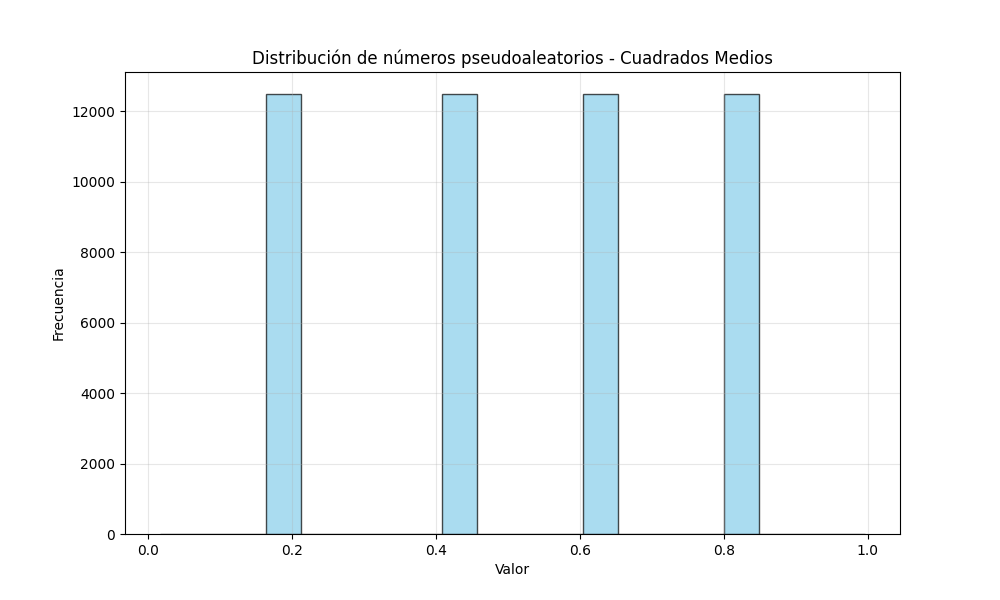
\includegraphics[width=0.6\textwidth]{Imagenes/distribucion_Cuadrados Medios.png}
\caption{------}
\end{figure}

\textbf{GCL tipo RANDU}

Aspecto esperado: Puede mostrar cierta uniformidad en una dimensión, pero las pruebas multidimensionales fallarán
Interpretación: El problema de RANDU no es evidente en un histograma unidimensional, lo que demuestra que las pruebas visuales unidimensionales son insuficientes para evaluar la calidad de un generador.

\begin{figure}[H]
\centering
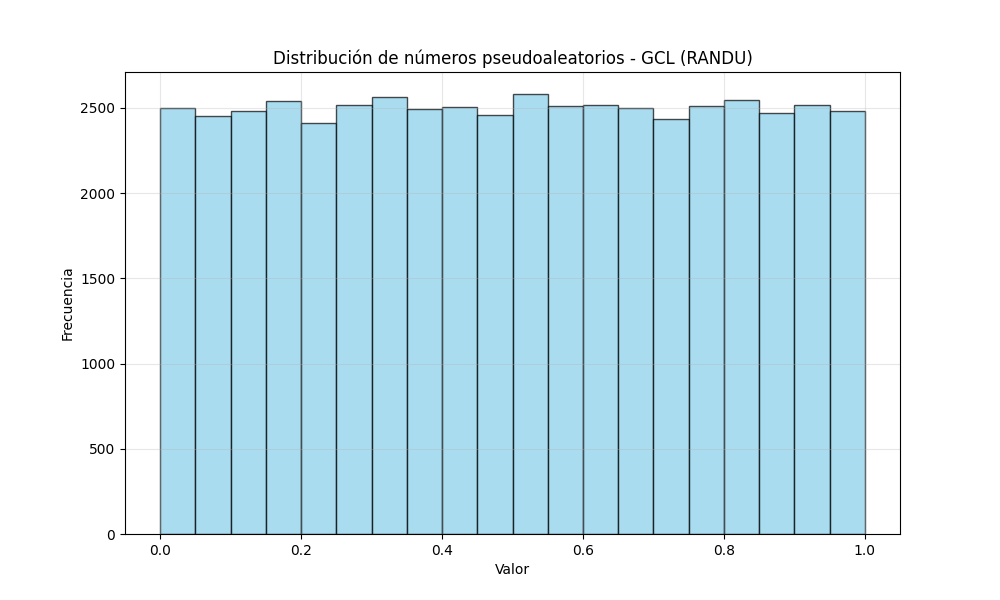
\includegraphics[width=0.6\textwidth]{Imagenes/distribucion_GCL (RANDU).png}
\caption{------}
\end{figure}

\textbf{NumPy Random}

Distribución muy cercana a una uniforme ideal. Esto confirma que NumPy utiliza un algoritmo de alta calidad (basado en Mersenne Twister), que pasa todas las pruebas estadísticas y visuales necesarias para su uso en simulación científica.

\begin{figure}[H]
\centering
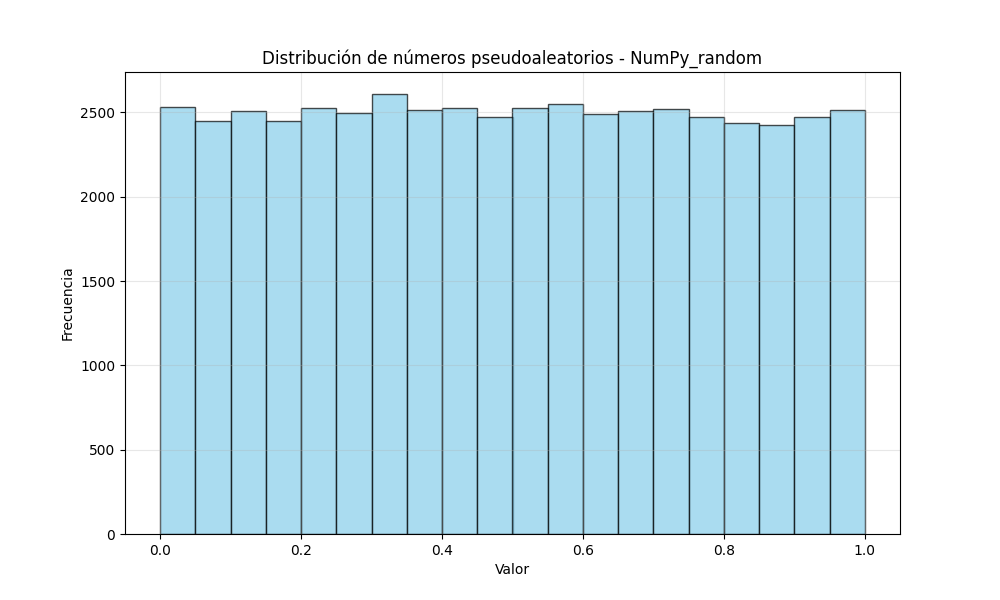
\includegraphics[width=0.6\textwidth]{Imagenes/distribucion_NumPy_random.png}
\caption{------}
\end{figure}

\textbf{Python Random}

Muestra una excelente cobertura del espacio [0,1). Es un generador robusto, adecuado para tareas generales de aleatoriedad. Se basa también en el Mersenne Twister, lo que garantiza buenas propiedades estadísticas.

\begin{figure}[H]
\centering
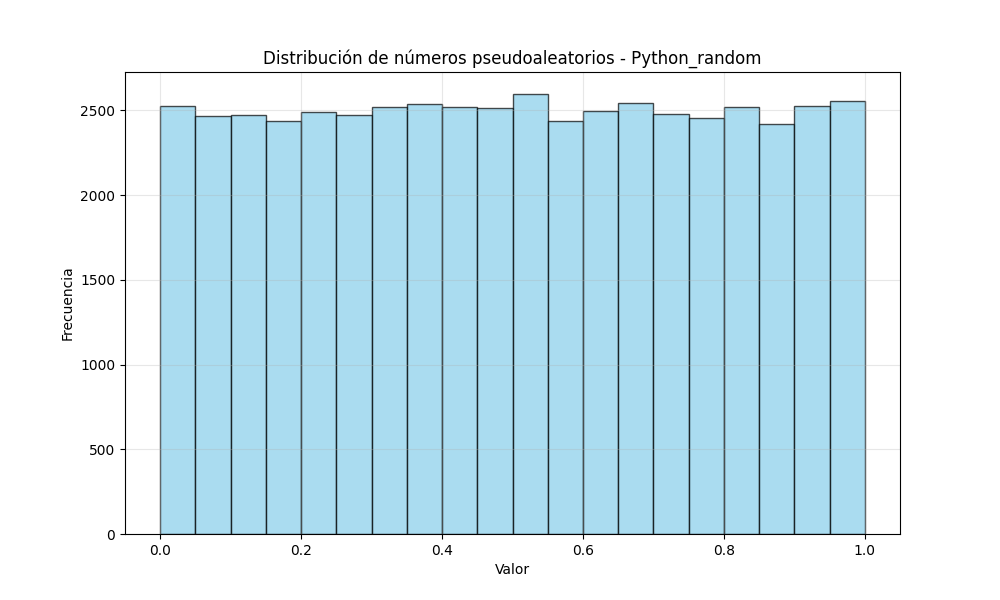
\includegraphics[width=0.6\textwidth]{Imagenes/distribucion_Python_random.png}
\caption{------}
\end{figure}

\textbf{Random.org}

Como se trata de números aleatorios obtenidos por fenómenos físicos reales, es lógico que su distribución sea excelente. Esta fuente es útil si se requiere aleatoriedad real, aunque su uso depende de conectividad externa.

\begin{figure}[H]
\centering
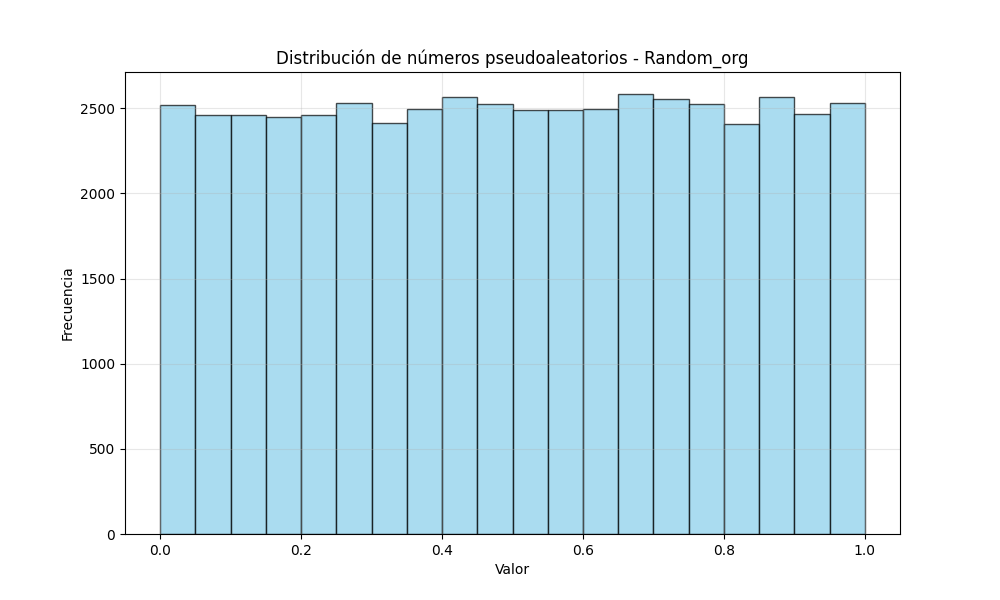
\includegraphics[width=0.6\textwidth]{Imagenes/distribucion_Random_org.png}
\caption{------}
\end{figure}

\subsubsection{Gráficos de Series (Dispersión 2D)}
Estos gráficos muestran pares consecutivos de valores (ri, ri+1).
Interpretación Ideal
En un buen generador, los puntos deberían cubrir uniformemente el plano unitario [0,1) × [0,1) sin mostrar patrones, rayas, rejillas o agrupaciones.
Interpretación por Generador
GCL con Buenos Parámetros

Aspecto esperado: Nube de puntos uniforme que cubre todo el plano
Interpretación: No hay correlación visible entre valores consecutivos, lo que indica buena independencia estadística.

\textbf{GCL tipo RANDU}

Aspecto esperado: Puede verse relativamente uniforme en 2D (aunque en 3D mostrará problemas severos)
Interpretación: El RANDU es famoso porque sus defectos no son evidentes en pruebas bidimensionales, pero son catastróficos en tres dimensiones.
\begin{figure}[H]
\centering
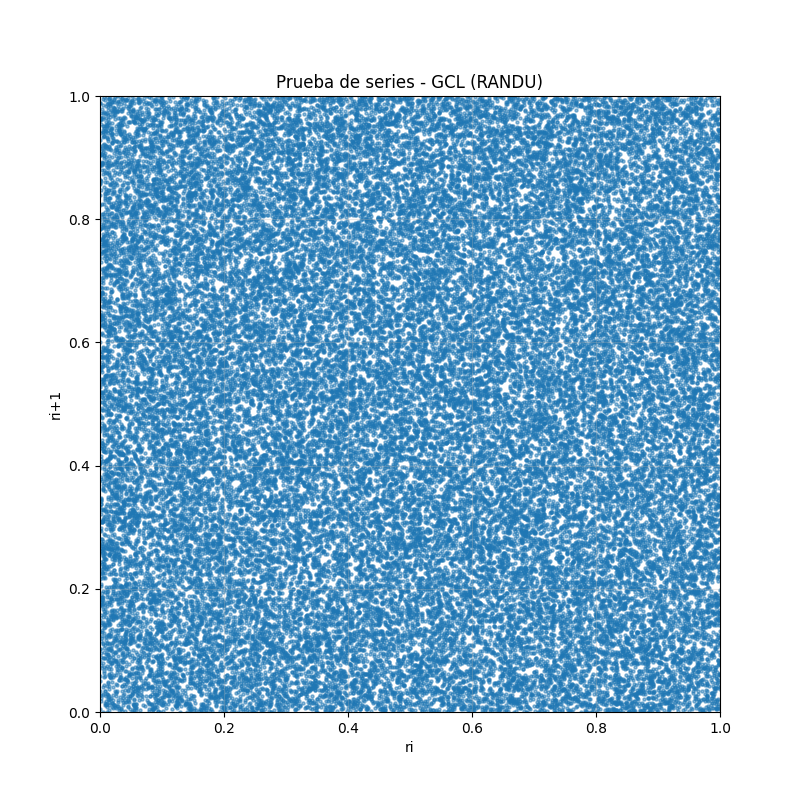
\includegraphics[width=0.6\textwidth]{Imagenes/series_GCL (RANDU).png}
\caption{GCL (RANDU)}
\end{figure}

\textbf{Cuadrados Medios}

Aspecto esperado: Puntos agrupados cerca del origen o formando patrones muy evidentes

Interpretación: Alta correlación entre valores consecutivos, lo que es una señal clara de pobre calidad del generador.
\begin{figure}[H]
\centering
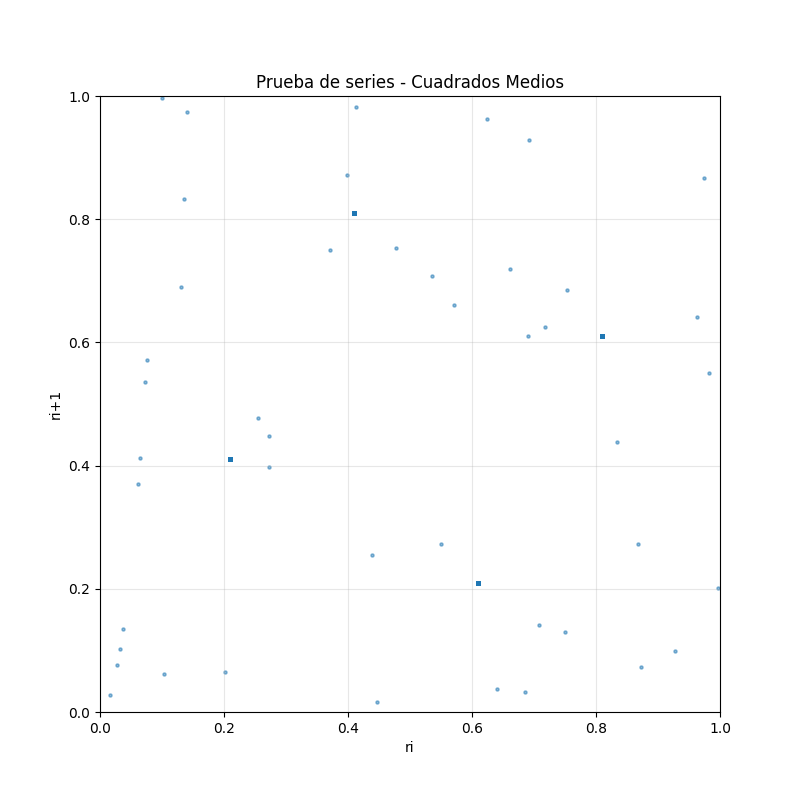
\includegraphics[width=0.6\textwidth]{Imagenes/series_Cuadrados Medios.png}
\caption{Cuadrados Medios}
\end{figure}
\textbf{Python Random | NumPy}

Aspecto esperado: Distribución uniforme sin patrones visibles
Interpretación: Ausencia de correlación entre valores consecutivos, indicando buena calidad.
\begin{figure}[H]
\centering
\begin{subfigure}[b]{0.45\textwidth}
    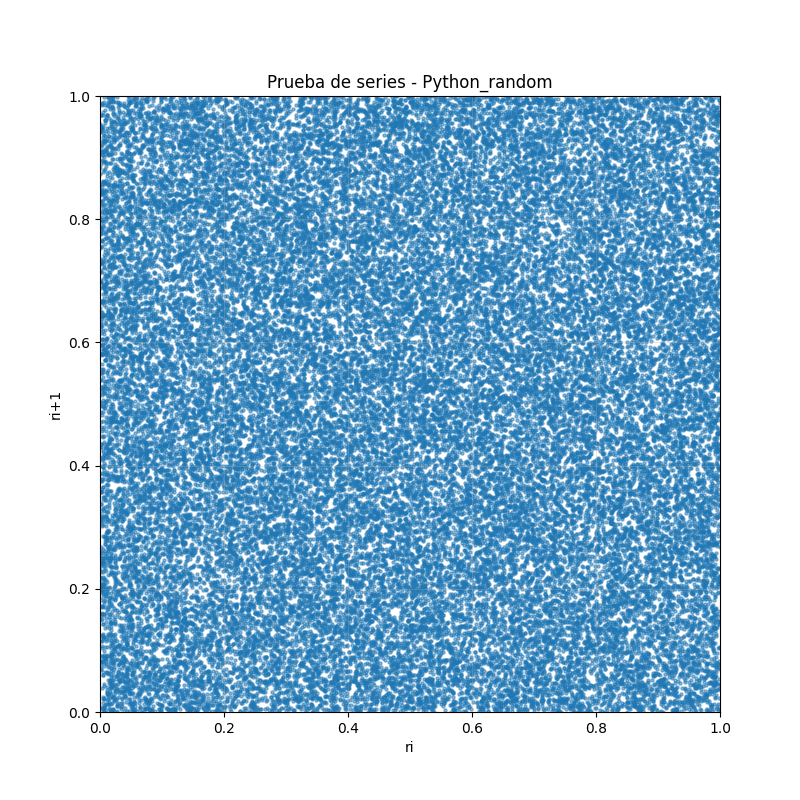
\includegraphics[width=\textwidth]{Imagenes/series_Python_random.png}
    \caption{Python Random}
\end{subfigure}
\hfill
\begin{subfigure}[b]{0.45\textwidth}
    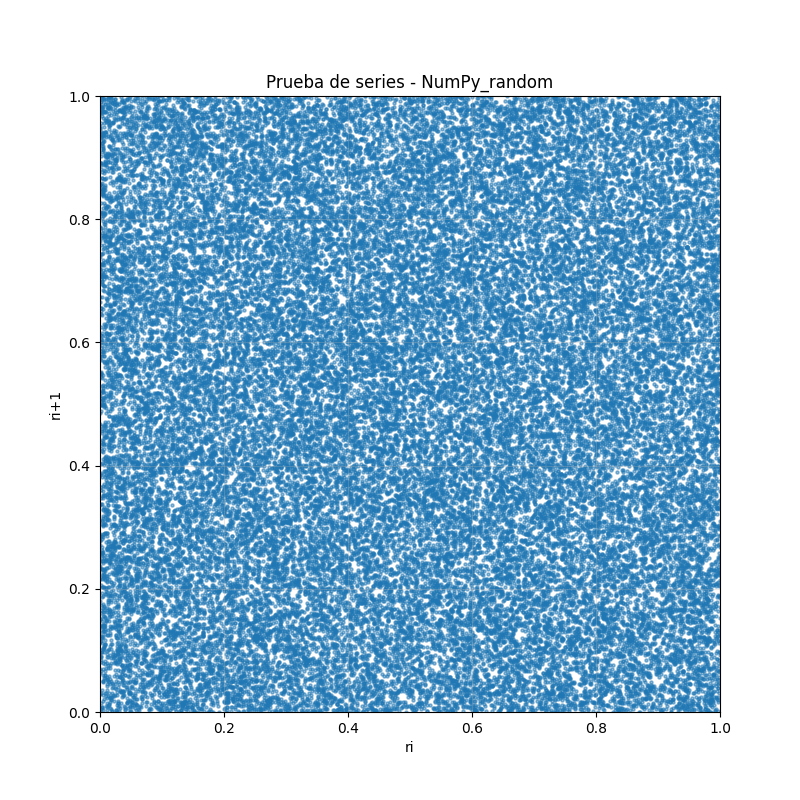
\includegraphics[width=\textwidth]{Imagenes/series_NumPy_random.png}
    \caption{NumPy Random}
\end{subfigure}
\caption{Figura X: Gráficos de autocorrelación – Python y NumPy}
\end{figure}

\subsubsection{Visualizaciones 3D}
Estos gráficos muestran ternas consecutivas de valores (ri, ri+1, ri+2).
Interpretación Ideal
Los puntos deberían distribuirse uniformemente en el cubo unitario sin formar patrones, planos o estructuras.
Interpretación por Generador
\textbf{GCL con Buenos Parámetros}

Aspecto esperado: Nube de puntos tridimensional uniforme
Interpretación: Buena independencia estadística incluso cuando se consideran tres valores consecutivos.

\textbf{GCL tipo RANDU}

Aspecto esperado: Puntos alineados en planos paralelos muy evidentes
Interpretación: Este es el famoso defecto del RANDU. Los puntos caen en exactamente 15 planos en el espacio 3D, lo que demuestra una correlación severa y predecible entre valores consecutivos. Es un ejemplo perfecto de cómo un generador puede pasar pruebas simples pero fallar espectacularmente en pruebas más sofisticadas.

\textbf{Cuadrados Medios}

Aspecto esperado: Concentración de puntos en una región pequeña o formando estructuras muy regulares
Interpretación: Alta correlación multidimensional, confirmando la mala calidad del generador.

\textbf{Python Random/NumPy}

Aspecto esperado: Distribución uniforme en todo el cubo
Interpretación: Los generadores modernos han sido diseñados específicamente para superar pruebas multidimensionales exigentes.

\begin{figure}[H]
\centering
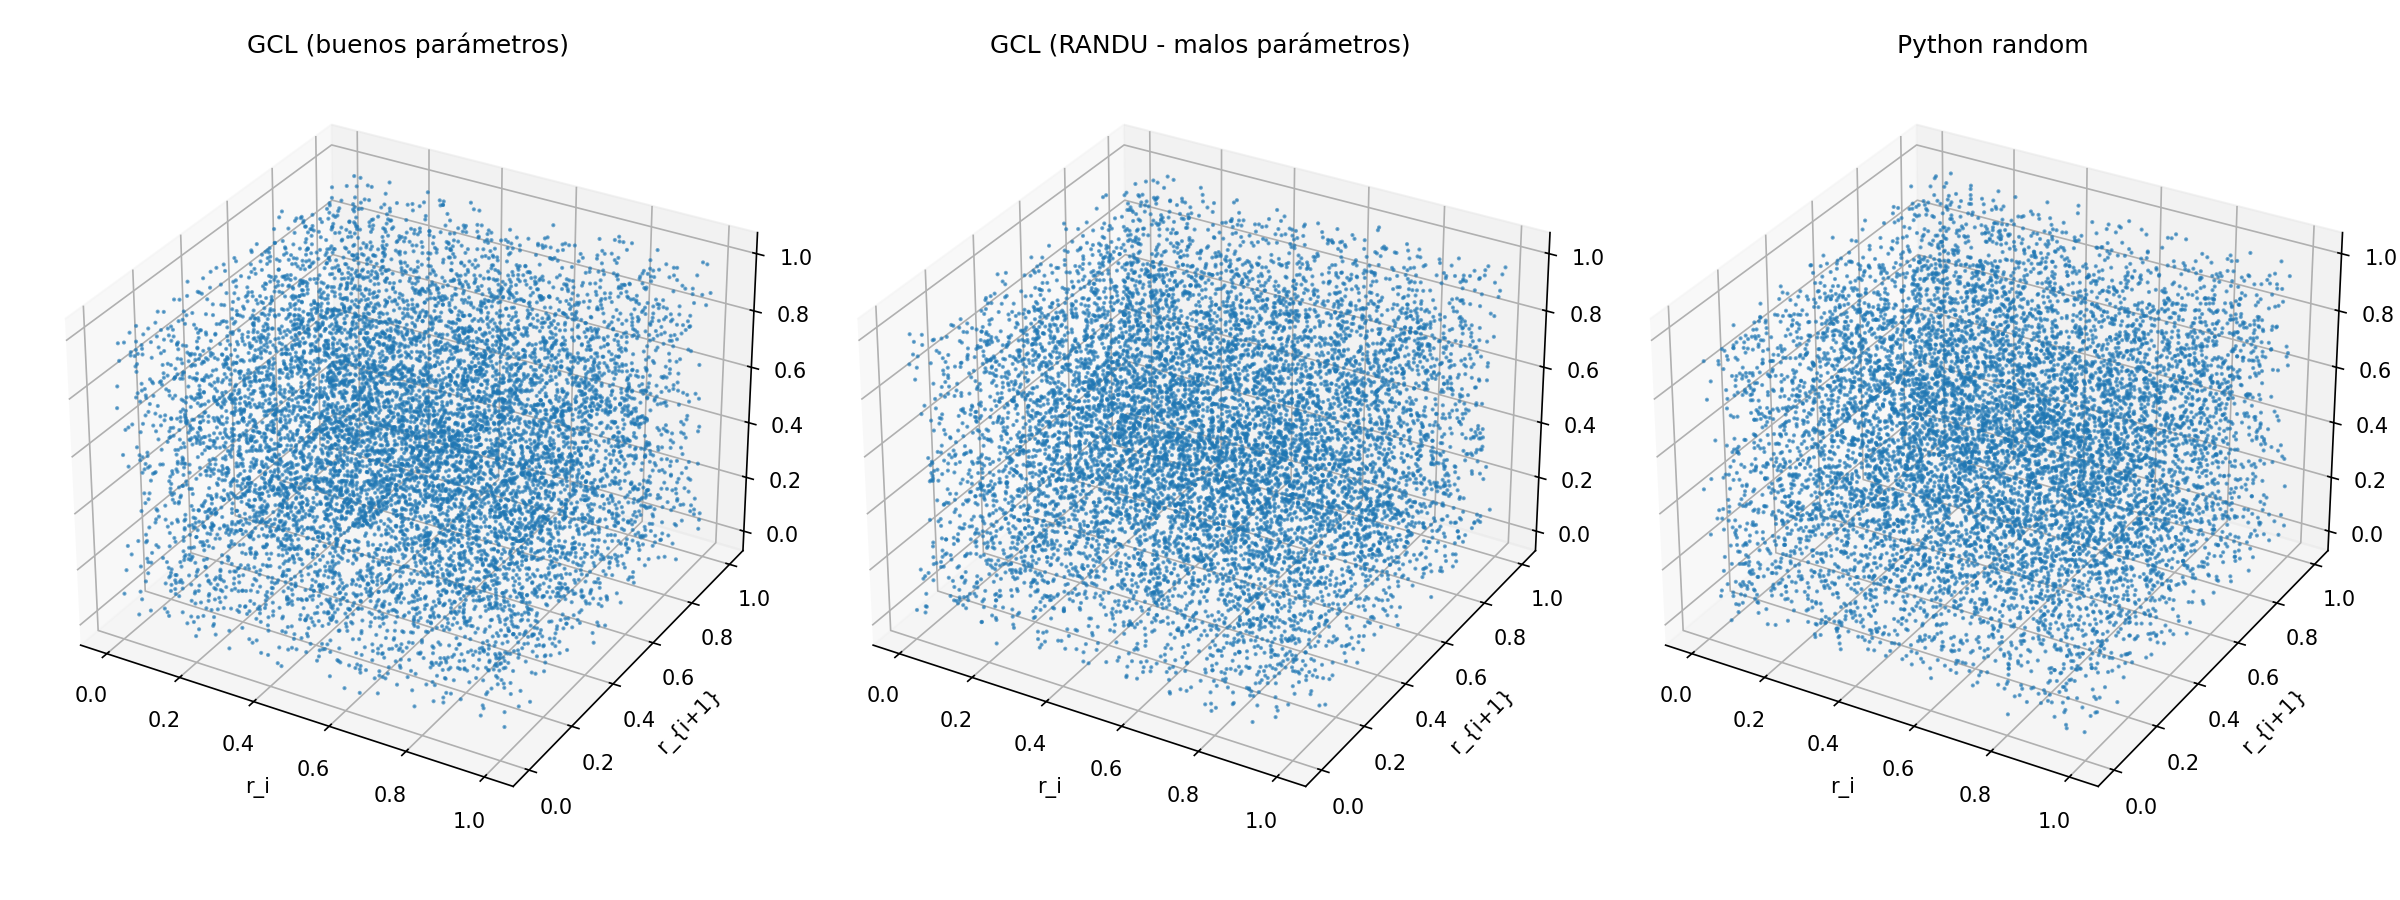
\includegraphics[width=0.85\textwidth]{Imagenes/comparacion_3d.png}
\caption{-----}
\end{figure}

\section{Autocorrelación y Evolución Temporal}

En esta sección analizamos la autocorrelación de los números generados por cada generador, junto con la evolución temporal de los valores producidos. Estas pruebas ayudan a detectar patrones o dependencias entre valores sucesivos que no deberían estar presentes en un buen generador de números pseudoaleatorios.

\subsection{Autocorrelación}

La prueba de autocorrelación mide el grado de dependencia lineal entre un valor y los valores anteriores de la secuencia. En un buen generador, se espera que las correlaciones sean cercanas a cero (excepto en el desfase cero).

\textbf{Cuadrados Medios:} Presenta valores de autocorrelación extremos, alternando entre 1 y -1, evidenciando una fuerte dependencia y comportamiento cíclico. Esto lo descalifica como un generador confiable.

\begin{figure}[H]
\centering
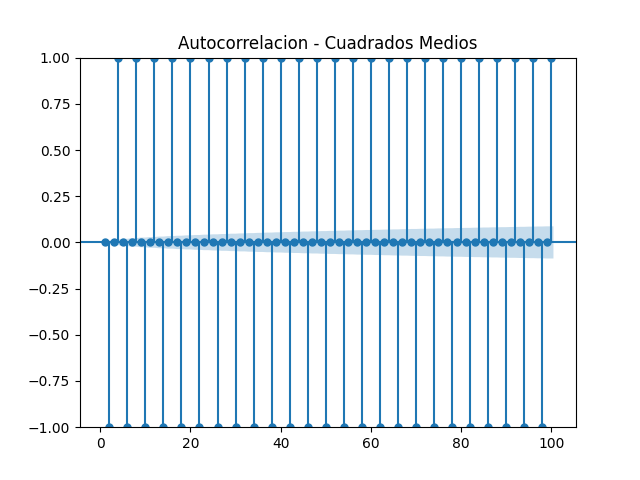
\includegraphics[width=0.6\textwidth]{Imagenes/autocorrelacion_Cuadrados Medios.png}
\caption{Autocorrelación – Cuadrados Medios}
\end{figure}

\textbf{GCL (buenos parámetros):} Muestra autocorrelaciones cercanas a cero, lo cual es deseable y refuerza su idoneidad para simulación.

\begin{figure}[H]
\centering
\includegraphics[width=0.6\textwidth]{Imagenes/autocorrelacion_GCL (buenos parámetros).png}
\caption{Autocorrelación – GCL (buenos parámetros)}
\end{figure}

\textbf{GCL (RANDU):} Aunque las correlaciones no son tan extremas como en Cuadrados Medios, mantiene valores bajos que podrían pasar desapercibidos en esta prueba, pero se evidenciarán problemas en otras dimensiones.

\begin{figure}[H]
\centering
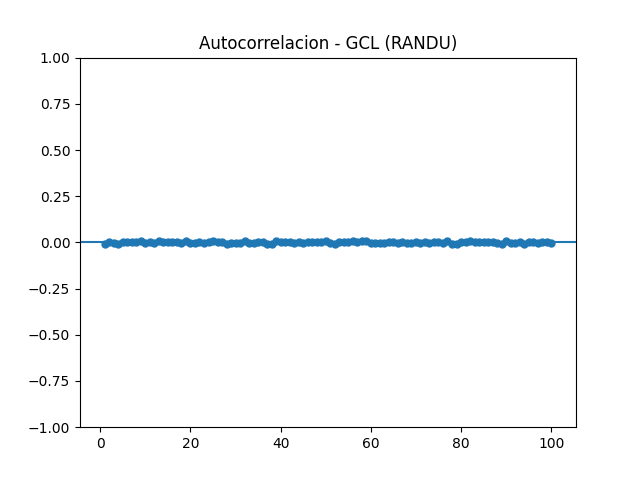
\includegraphics[width=0.6\textwidth]{Imagenes/autocorrelacion_GCL (RANDU).png}
\caption{Autocorrelación – GCL (RANDU)}
\end{figure}

\textbf{Python Random:} Se observa una buena dispersión sin patrones visibles, con autocorrelaciones cercanas a cero.

\begin{figure}[H]
\centering
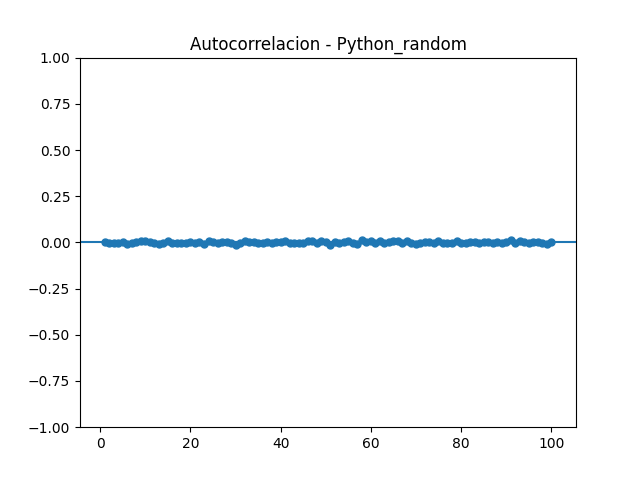
\includegraphics[width=0.6\textwidth]{Imagenes/autocorrelacion_Python_random.png}
\caption{Autocorrelación – Python Random}
\end{figure}

\textbf{NumPy Random:} Muestra comportamiento similar al anterior, con autocorrelaciones cercanas a cero y sin estructura.

\begin{figure}[H]
\centering
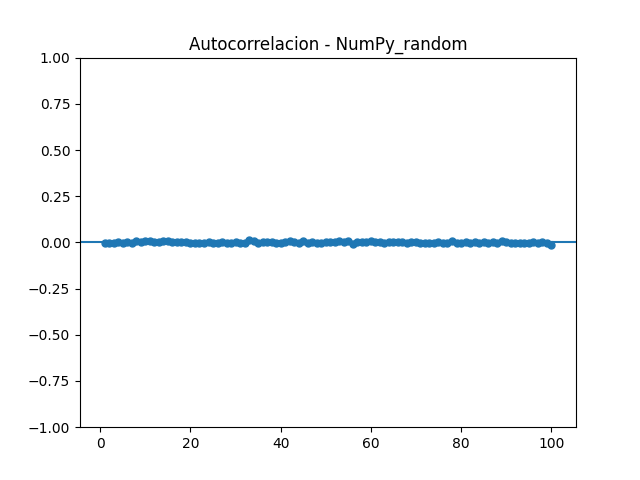
\includegraphics[width=0.6\textwidth]{Imagenes/autocorrelacion_NumPy_random.png}
\caption{Autocorrelación – NumPy Random}
\end{figure}

\textbf{Random.org:} Al provenir de un generador aleatorio verdadero, sus autocorrelaciones son mínimas y distribuidas sin tendencia.

\begin{figure}[H]
\centering
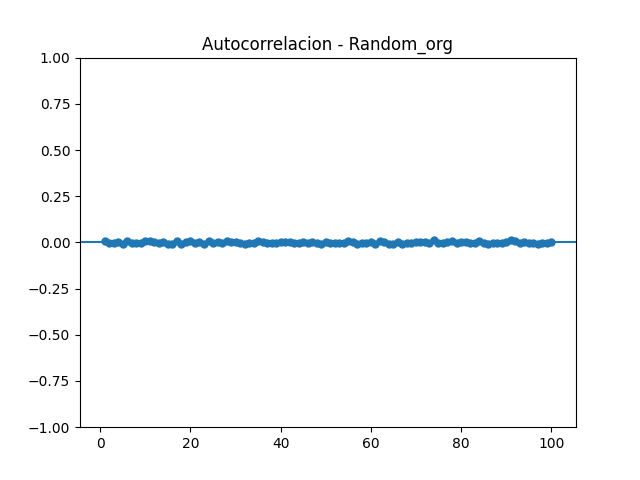
\includegraphics[width=0.6\textwidth]{Imagenes/autocorrelacion_Random_org.png}
\caption{Autocorrelación – Random.org}
\end{figure}

\subsection{Evolución Temporal de Cuadrados Medios}

Este gráfico muestra cómo los valores generados por el método de los Cuadrados Medios tienden a estabilizarse rápidamente en pocos valores, lo que evidencia su escasa capacidad para producir variabilidad. Esto coincide con la observación previa de que este método tiende a colapsar en ciclos muy cortos o valores fijos, comprometiendo gravemente la aleatoriedad de la secuencia.

\begin{figure}[H]
\centering
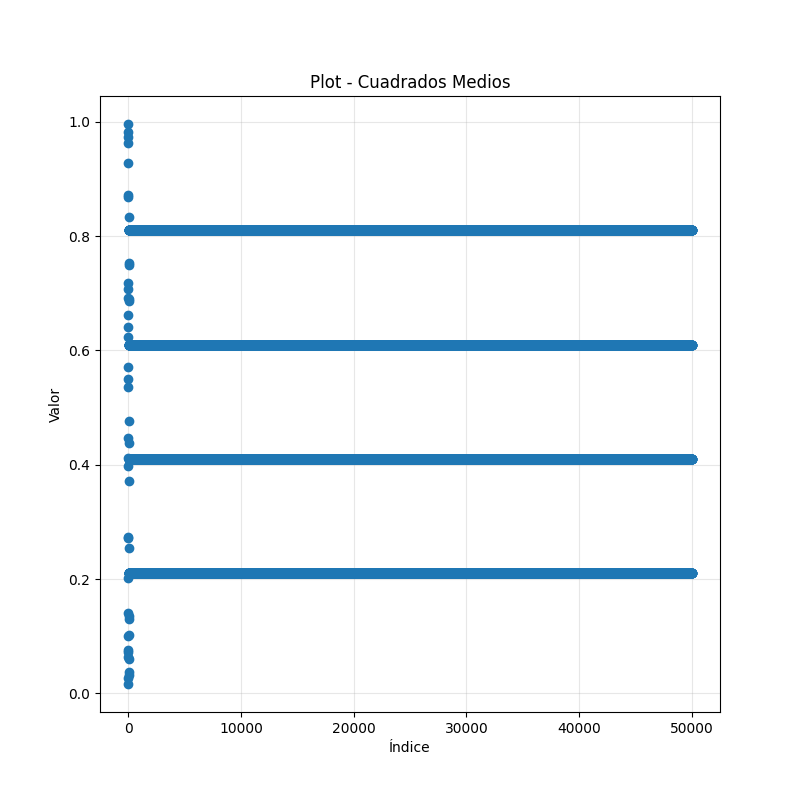
\includegraphics[width=0.6\textwidth]{Imagenes/plot_Cuadrados Medios.png}
\caption{Evolución del valor en función del índice para Cuadrados Medios}
\end{figure}

\section{Conclusión}
El análisis realizado evidencia que no todos los generadores de números pseudoaleatorios son adecuados para simulaciones. Métodos históricos como Cuadrados Medios y el GCL con parámetros tipo RANDU presentan comportamientos claramente deficientes, los cuales se reflejan tanto en pruebas estadísticas como en gráficos de distribución, series y autocorrelación. Estos generadores no logran reproducir la variabilidad esperada, mostrando patrones, ciclos cortos o concentraciones de valores que comprometen su utilidad en contextos de simulación.

Por el contrario, los generadores modernos como Python random, numpy.random y Random.org mostraron un desempeño robusto, generando secuencias bien distribuidas, sin correlaciones visibles y con una calidad estadística adecuada. Este contraste deja en evidencia por qué los métodos modernos superan ampliamente a los enfoques clásicos.

Además, el caso particular del generador RANDU demuestra la importancia de aplicar pruebas en múltiples dimensiones, ya que algunas deficiencias sólo se manifiestan en contextos tridimensionales. También se destaca la correlación entre los análisis gráficos y las pruebas estadísticas, que deben emplearse de forma complementaria. Por último, incluso dentro de una misma familia de algoritmos, como los GCL, la correcta elección de parámetros es fundamental para garantizar la calidad del generador.

\bibliographystyle{unsrt}  
\begin{thebibliography}{99}

\bibitem{simulaciongithub}
Aldana Risso Patrón. \textit{TP 2.1 - Generadores Pseudoaleatorios}.\\
Disponible en: \url{https://github.com/AldanaRP/TPSimulacion}


\bibitem{bacchini2018}  
Bacchini, H. \textit{Introducción a la Probabilidad y a la Estadística}.\\
Universidad de Buenos Aires, Facultad de Ciencias Económicas, 2018.\\
Disponible en: \url{http://bibliotecadigital.econ.uba.ar/download/libros/Bacchini_Introduccion-a-la-probabilidad-y-a-la-estadistica-2018.pdf}

\bibitem{numpyfromw3schools}
W3Schools \textit{NumPy Random Module for Python}.\\
Disponible en: \url{https://www.w3schools.com/python/numpy/numpy_random.asp}

\bibitem{statisticaltestpaper}
 Nist Paper\textit{A Statistical Test Suite for Random and Pseudorandom Number Generators for Cryptographic Applications(Paper)}.\\
Disponible en: \url{https://www.nist.gov/publications/statistical-test-suite-random-and-pseudorandom-number-generators-cryptographic}

\end{thebibliography}

\end{document}
